\chapter{Experiments}
\label{ch:experiments}
\section{NAO}
Brief description of NAO v5 (which is running BHuman).

\section{Simple Staircase}
Staircase from 1cm to 5cm. Limitations of the robot.
\begin{figure}
  \centering
  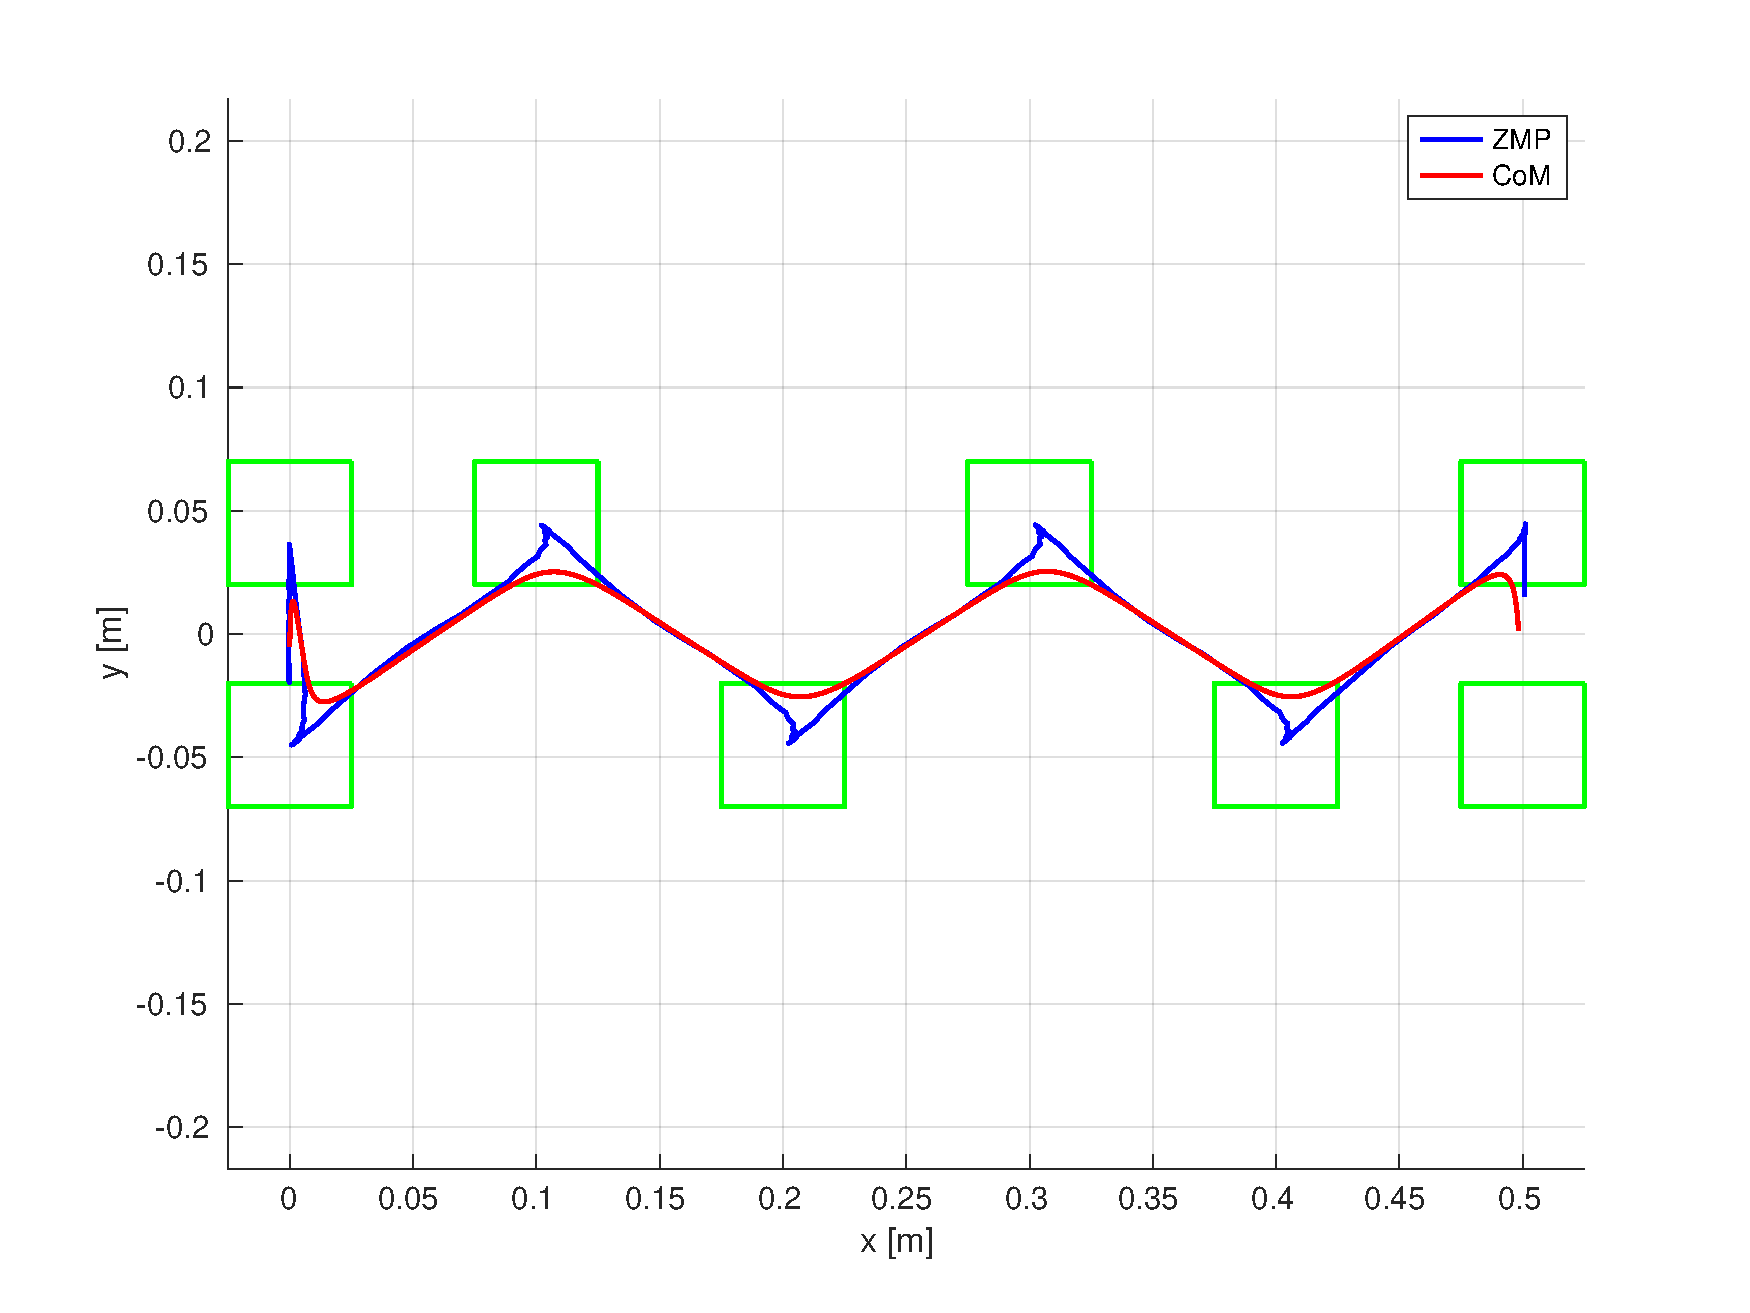
\includegraphics[width=\textwidth]
      {figures/experiments/simple-staircase/xy-plot-4cm.pdf}
  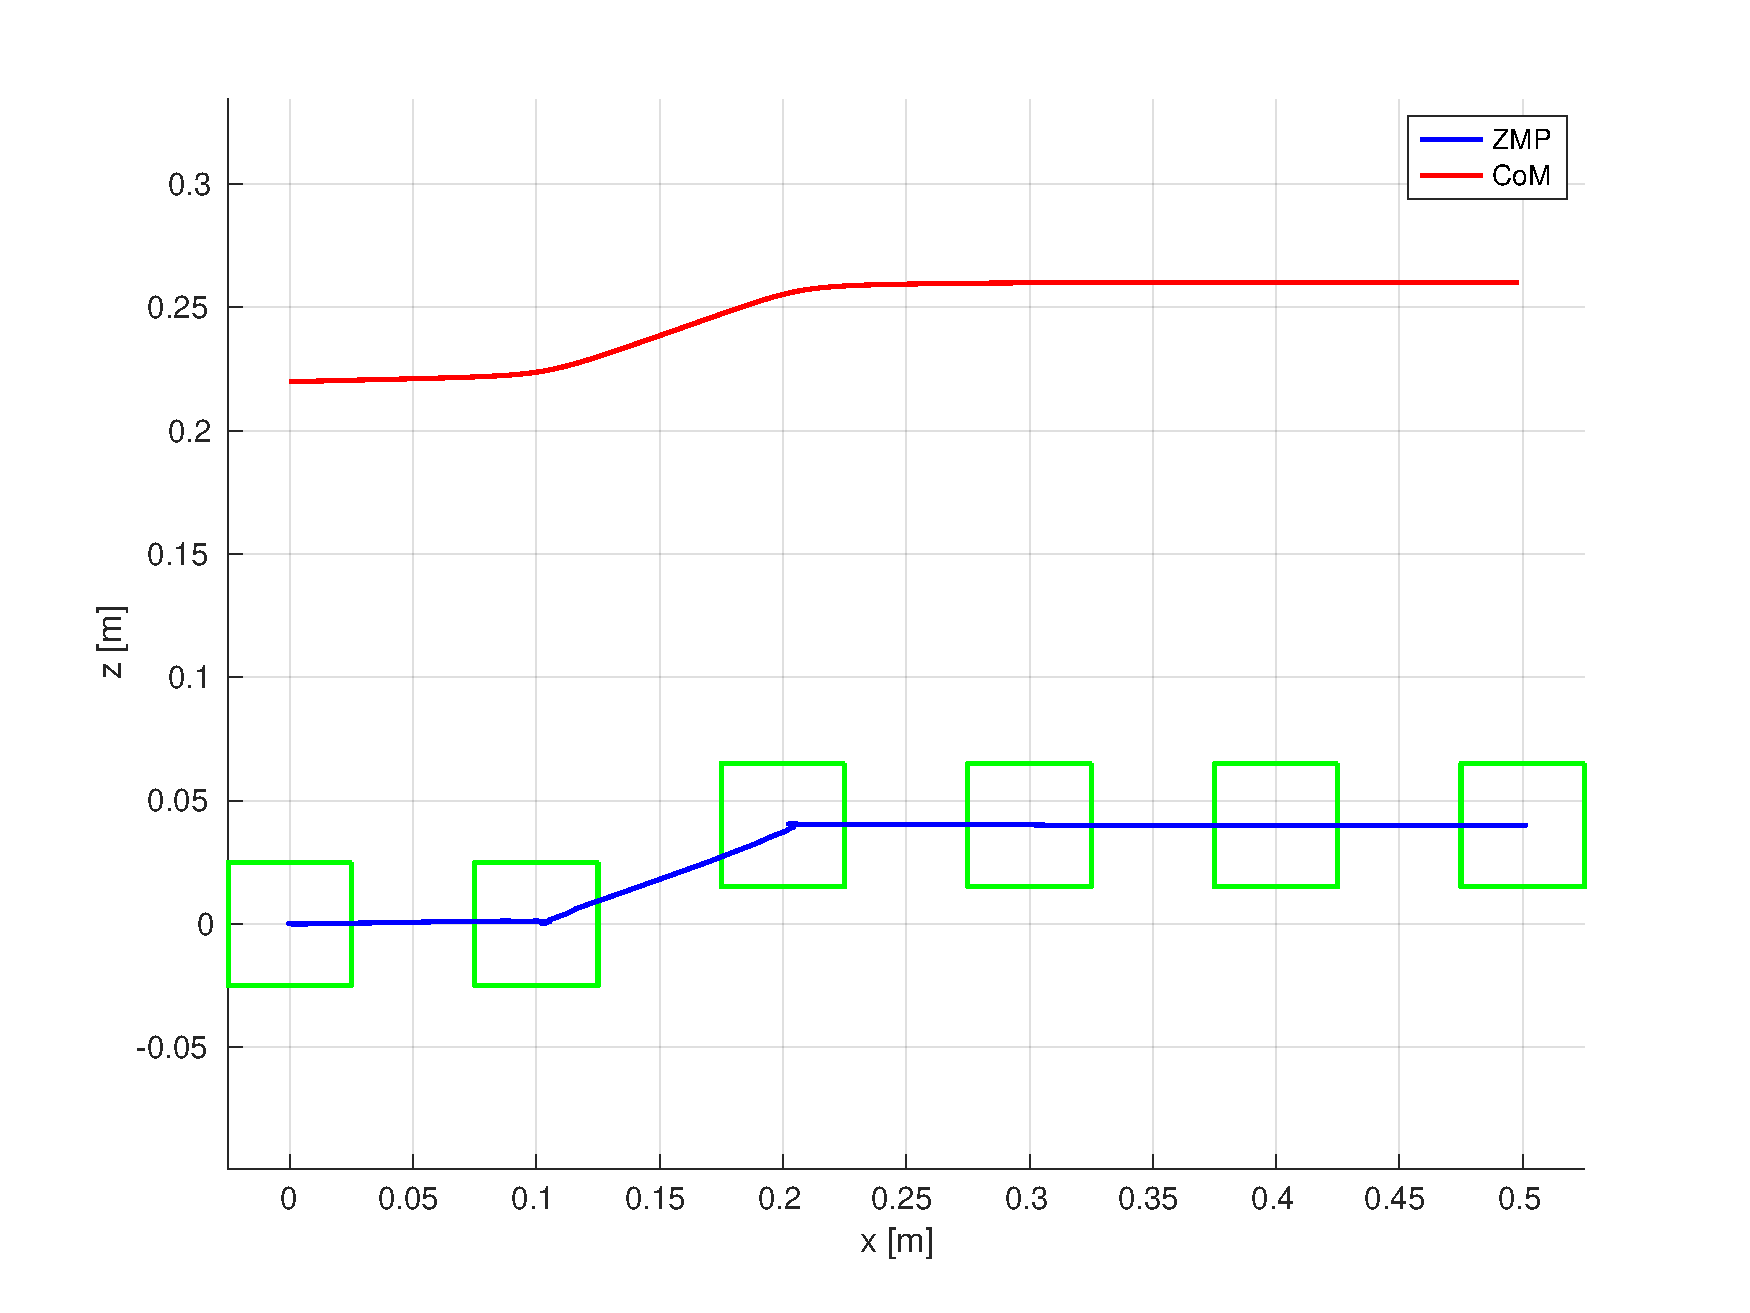
\includegraphics[width=\textwidth]
      {figures/experiments/simple-staircase/xz-plot-4cm.pdf}
  \caption{The plots show how the CoM and the ZMP vary with respect to the
		footsteps in the scenario ``Simple Staircase''.
    The green boxes represent the footsteps.}
  \label{fig:experiments:simple-staircase:comzmp}
\end{figure}

\section{Multiple Staircases}
Two consecutive staircases of 2cm.

\subsection{Upstairs}
Upstairs.
\begin{figure}
  \centering
  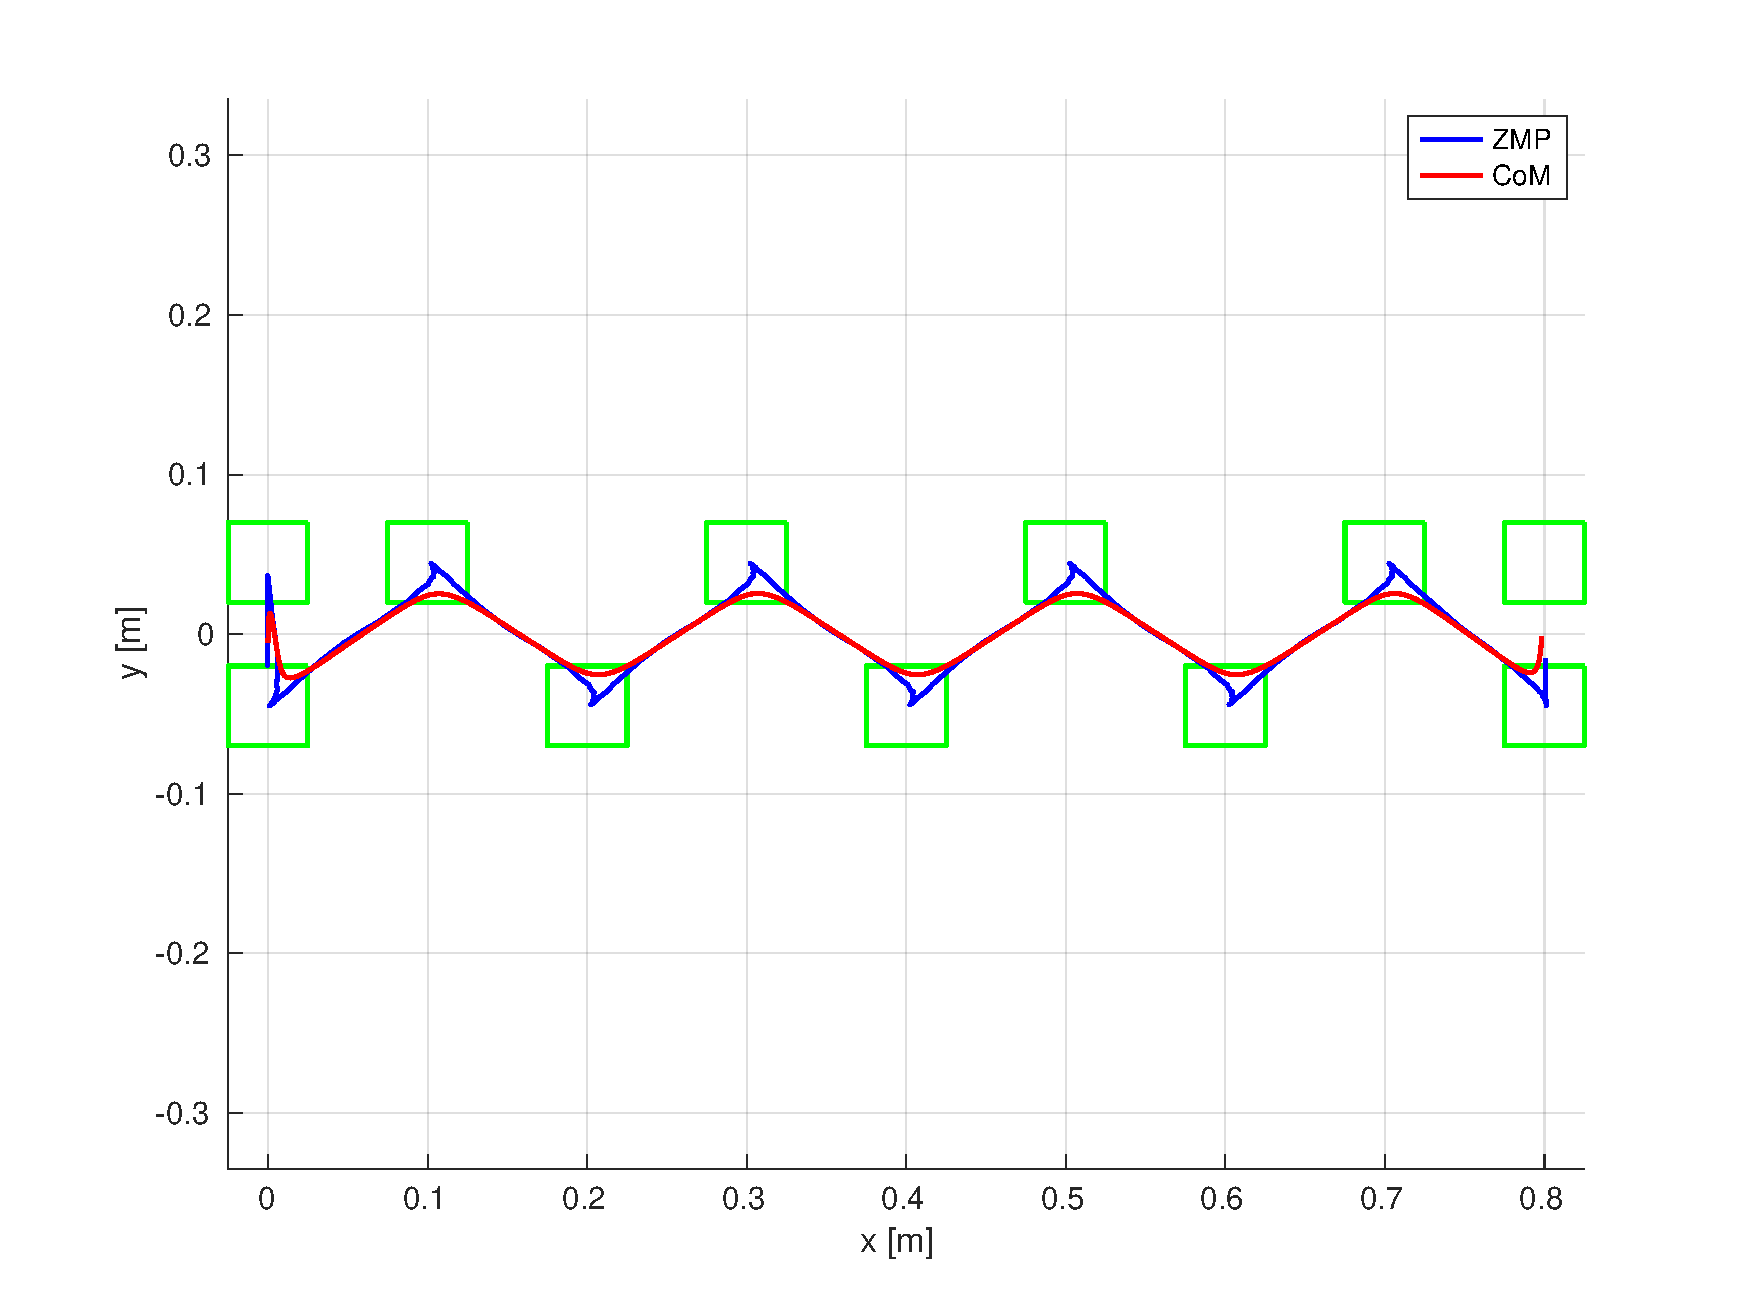
\includegraphics[width=\textwidth]
      {figures/experiments/multiple-staircases/upstairs/xy-plot-2cm.pdf}
  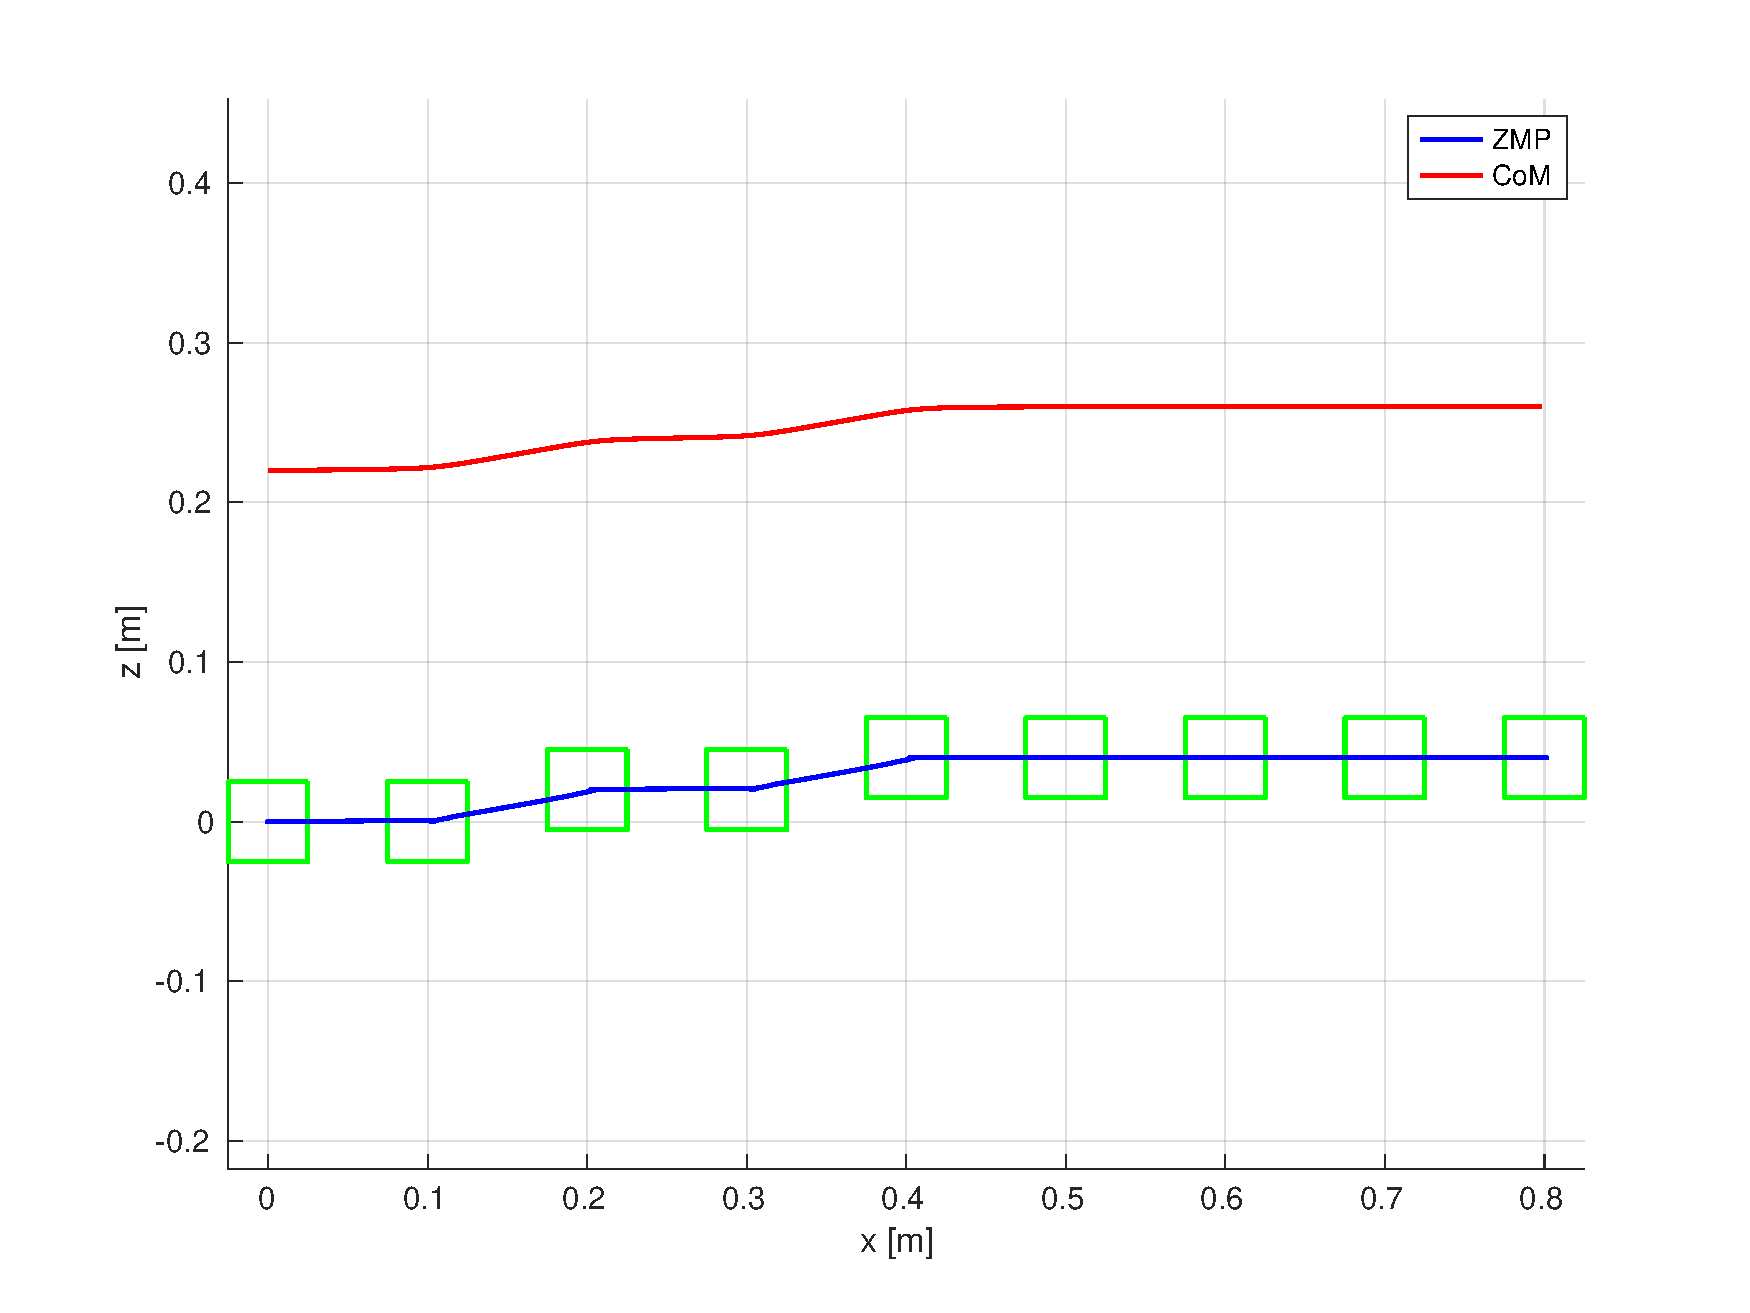
\includegraphics[width=\textwidth]
      {figures/experiments/multiple-staircases/upstairs/xz-plot-2cm.pdf}
  \caption{The plots show how the CoM and the ZMP vary with respect to the
		footsteps in the scenario ``Multiple Staircases (Upstairs)''.
    The green boxes represent the footsteps.}
  \label{fig:experiments:multiple-staircases:upstairs:comzmp}
\end{figure}

\subsection{Downstairs}
Downstairs.
\begin{figure}
  \centering
  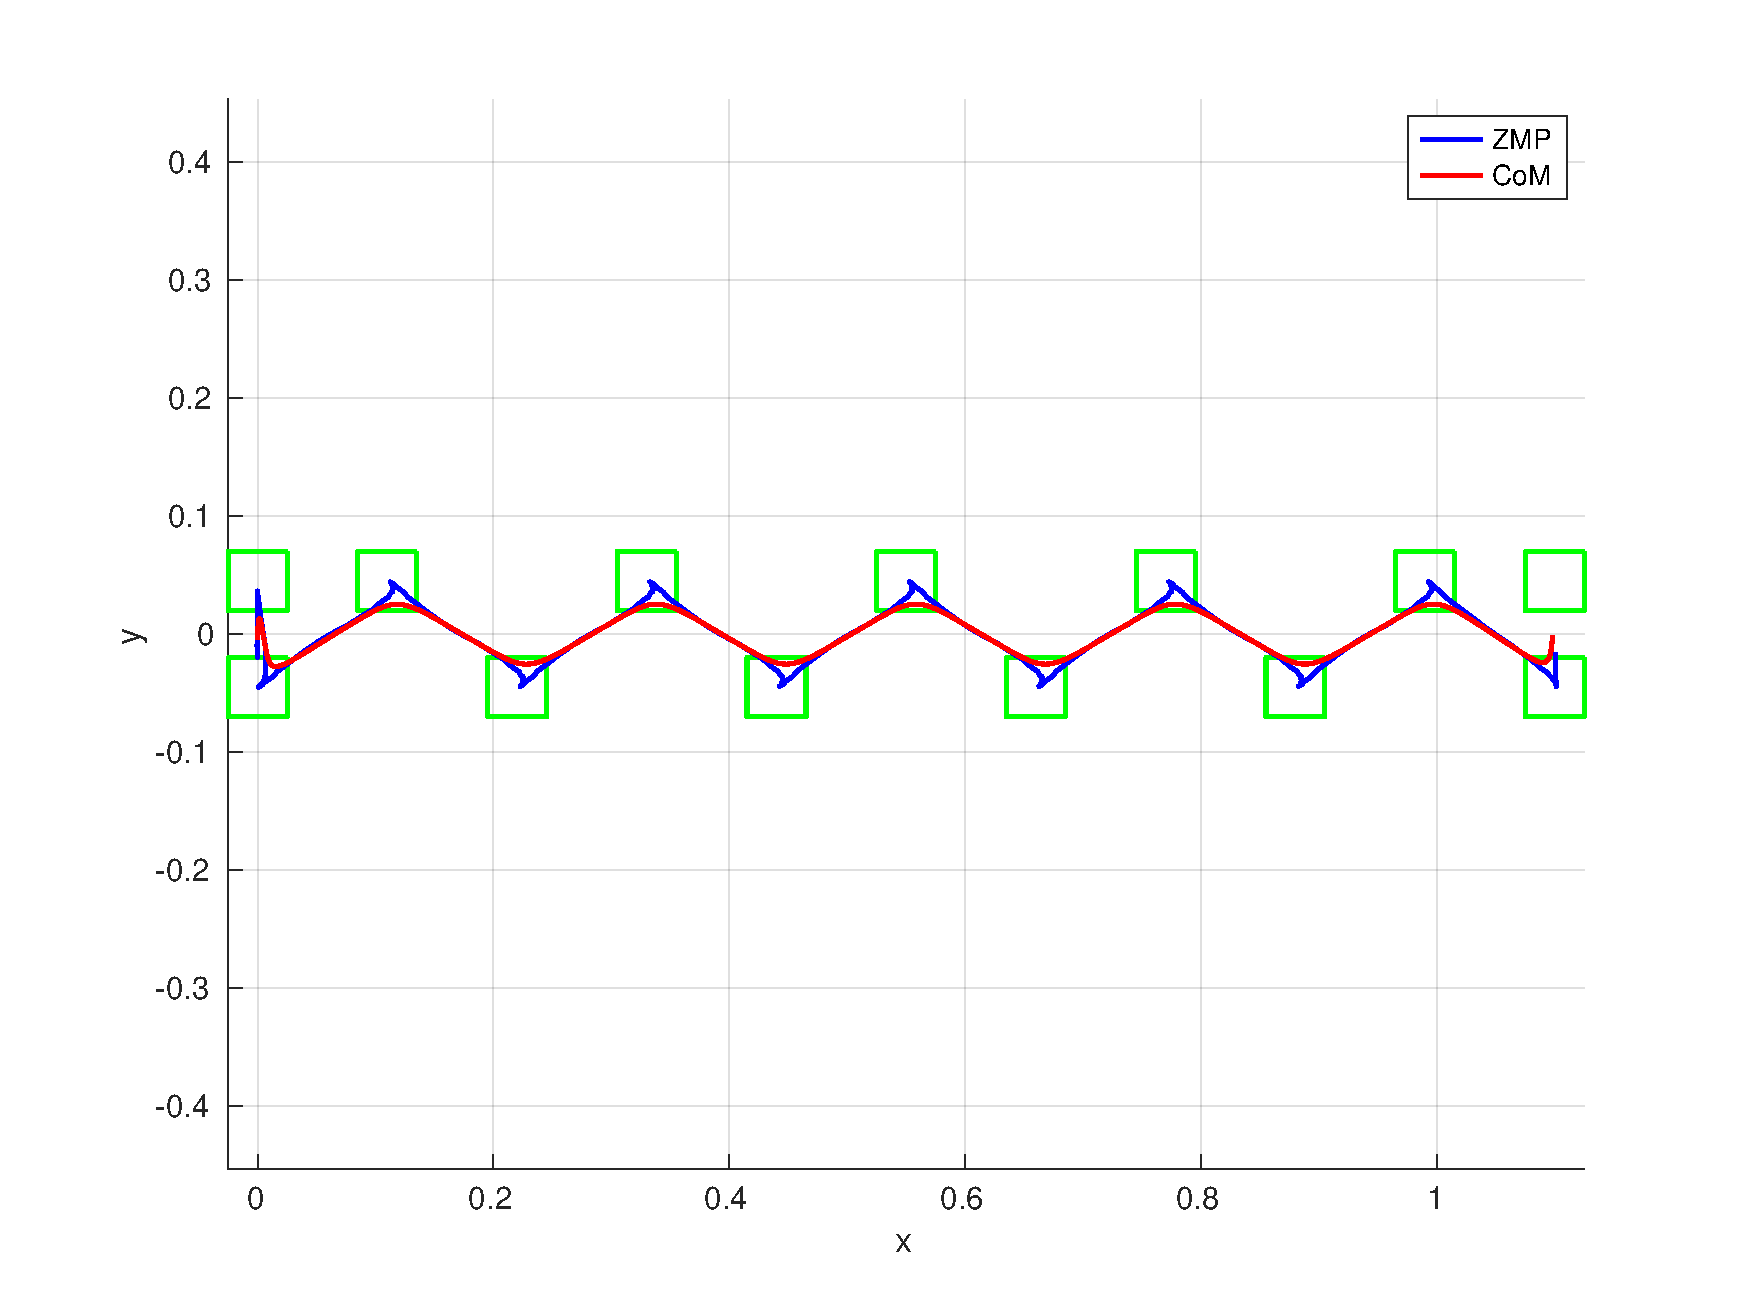
\includegraphics[width=\textwidth]
      {figures/experiments/multiple-staircases/downstairs/xy-plot-2cm.pdf}
  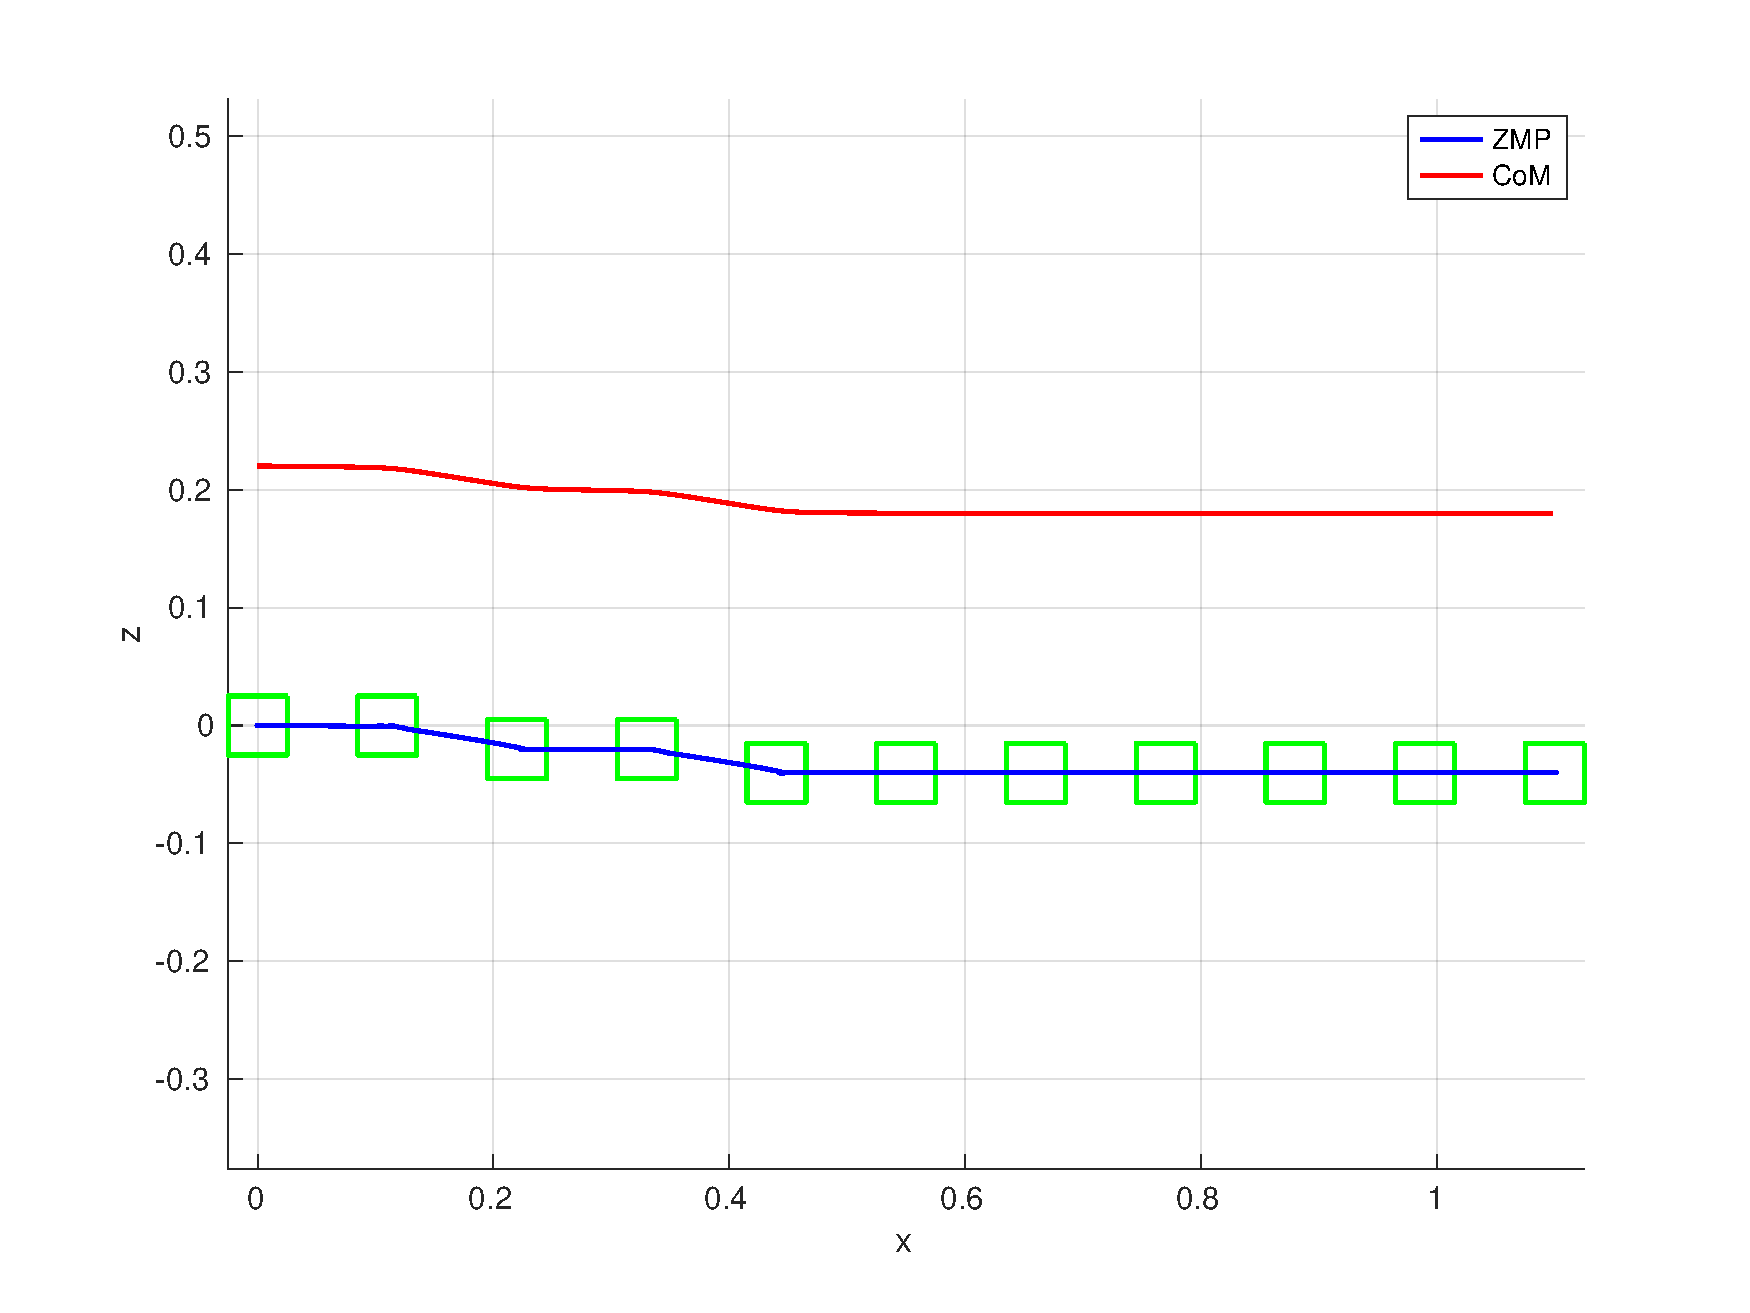
\includegraphics[width=\textwidth]
      {figures/experiments/multiple-staircases/downstairs/xz-plot-2cm.pdf}
  \caption{The plots show how the CoM and the ZMP vary with respect to the
		footsteps in the scenario ``Multiple Staircases (Downstairs)''.
    The green boxes represent the footsteps.}
  \label{fig:experiments:multiple-staircases:downstairs:comzmp}
\end{figure}

\section{Obstacle Avoidance}
Footstep planning with manually generated elevation mapping. Map contains 
an obstacle that can not be climbed by NAO because of short legs.
\begin{figure}
    \centering
    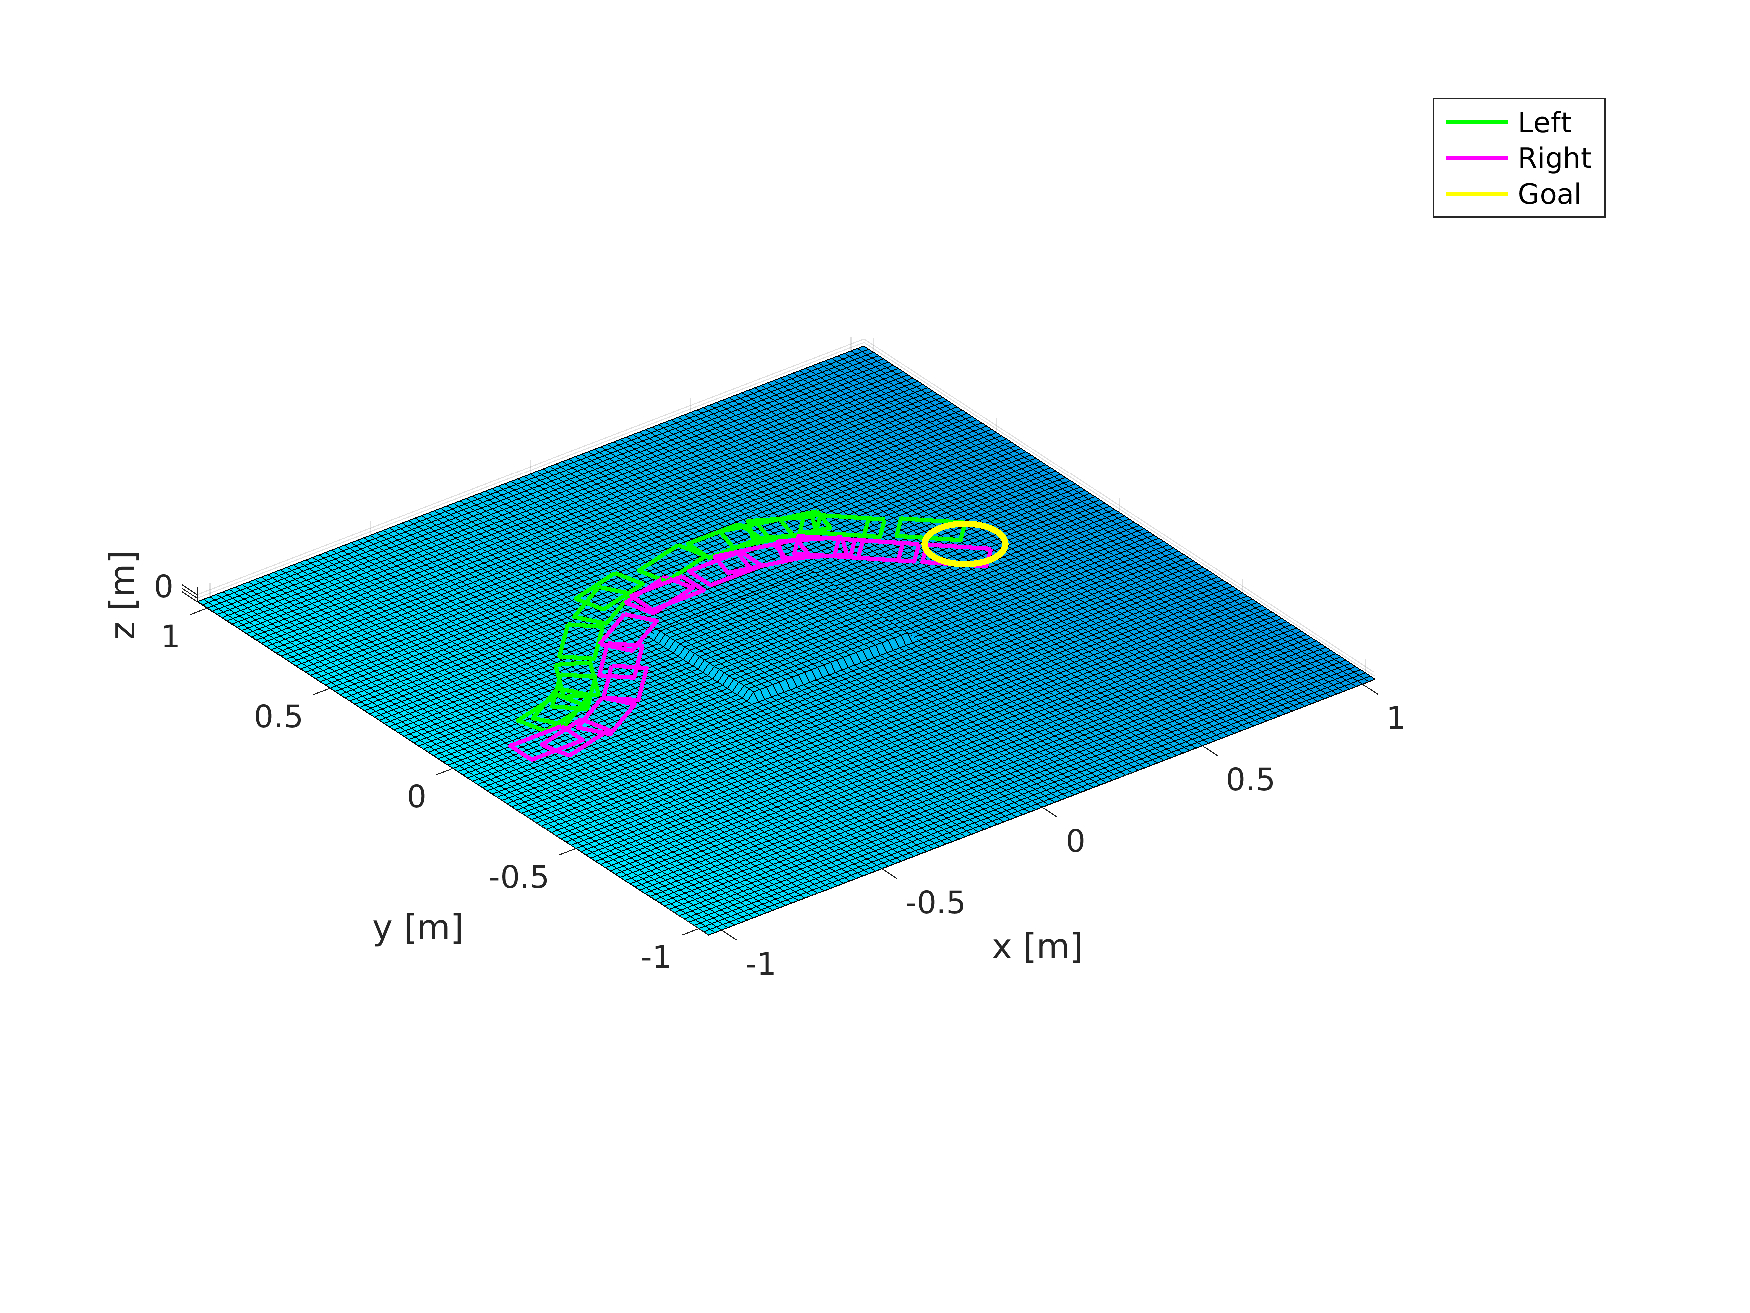
\includegraphics[width=0.95\textwidth]
        {figures/experiments/obstacle-avoidance/footstep-plan.pdf}
    \caption{Footstep plan generated for the scenario ``Obstacle Avoidance''.}
    \label{fig:experiments:obstacle-avoidance:footstep-plan}
\end{figure}
\begin{figure}
    \centering
    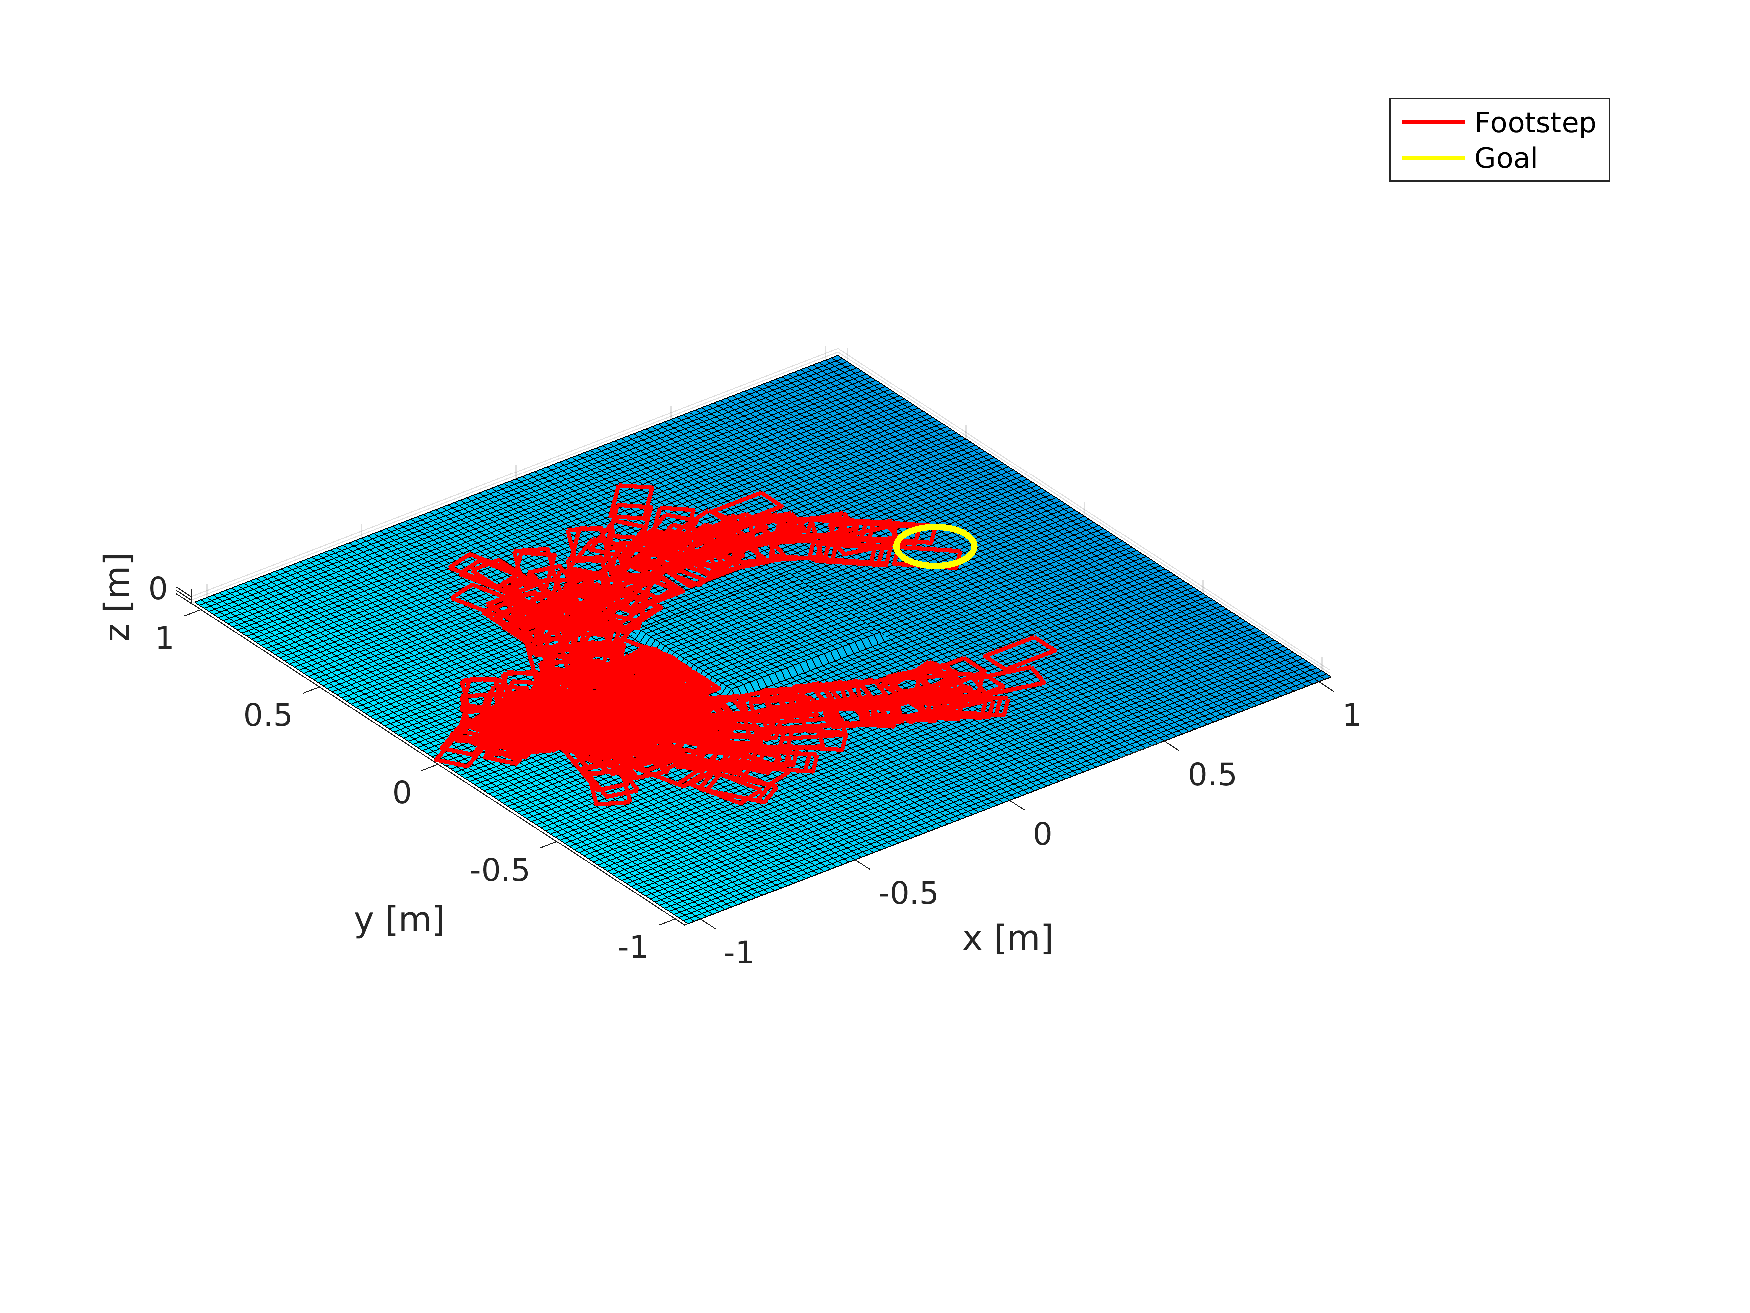
\includegraphics[width=0.95\textwidth]
        {figures/experiments/obstacle-avoidance/rrt-tree.pdf}
    \caption{Tree generated for the scenario ``Obstacle Avoidance''.}
    \label{fig:experiments:obstacle-avoidance:rrt-tree}
\end{figure}

\section{Stair Climbing in Unknown Environment}
Stair climbing (unknown environment). Planner + \texttt{elevation\_mapping}.
\begin{figure}
    \centering
    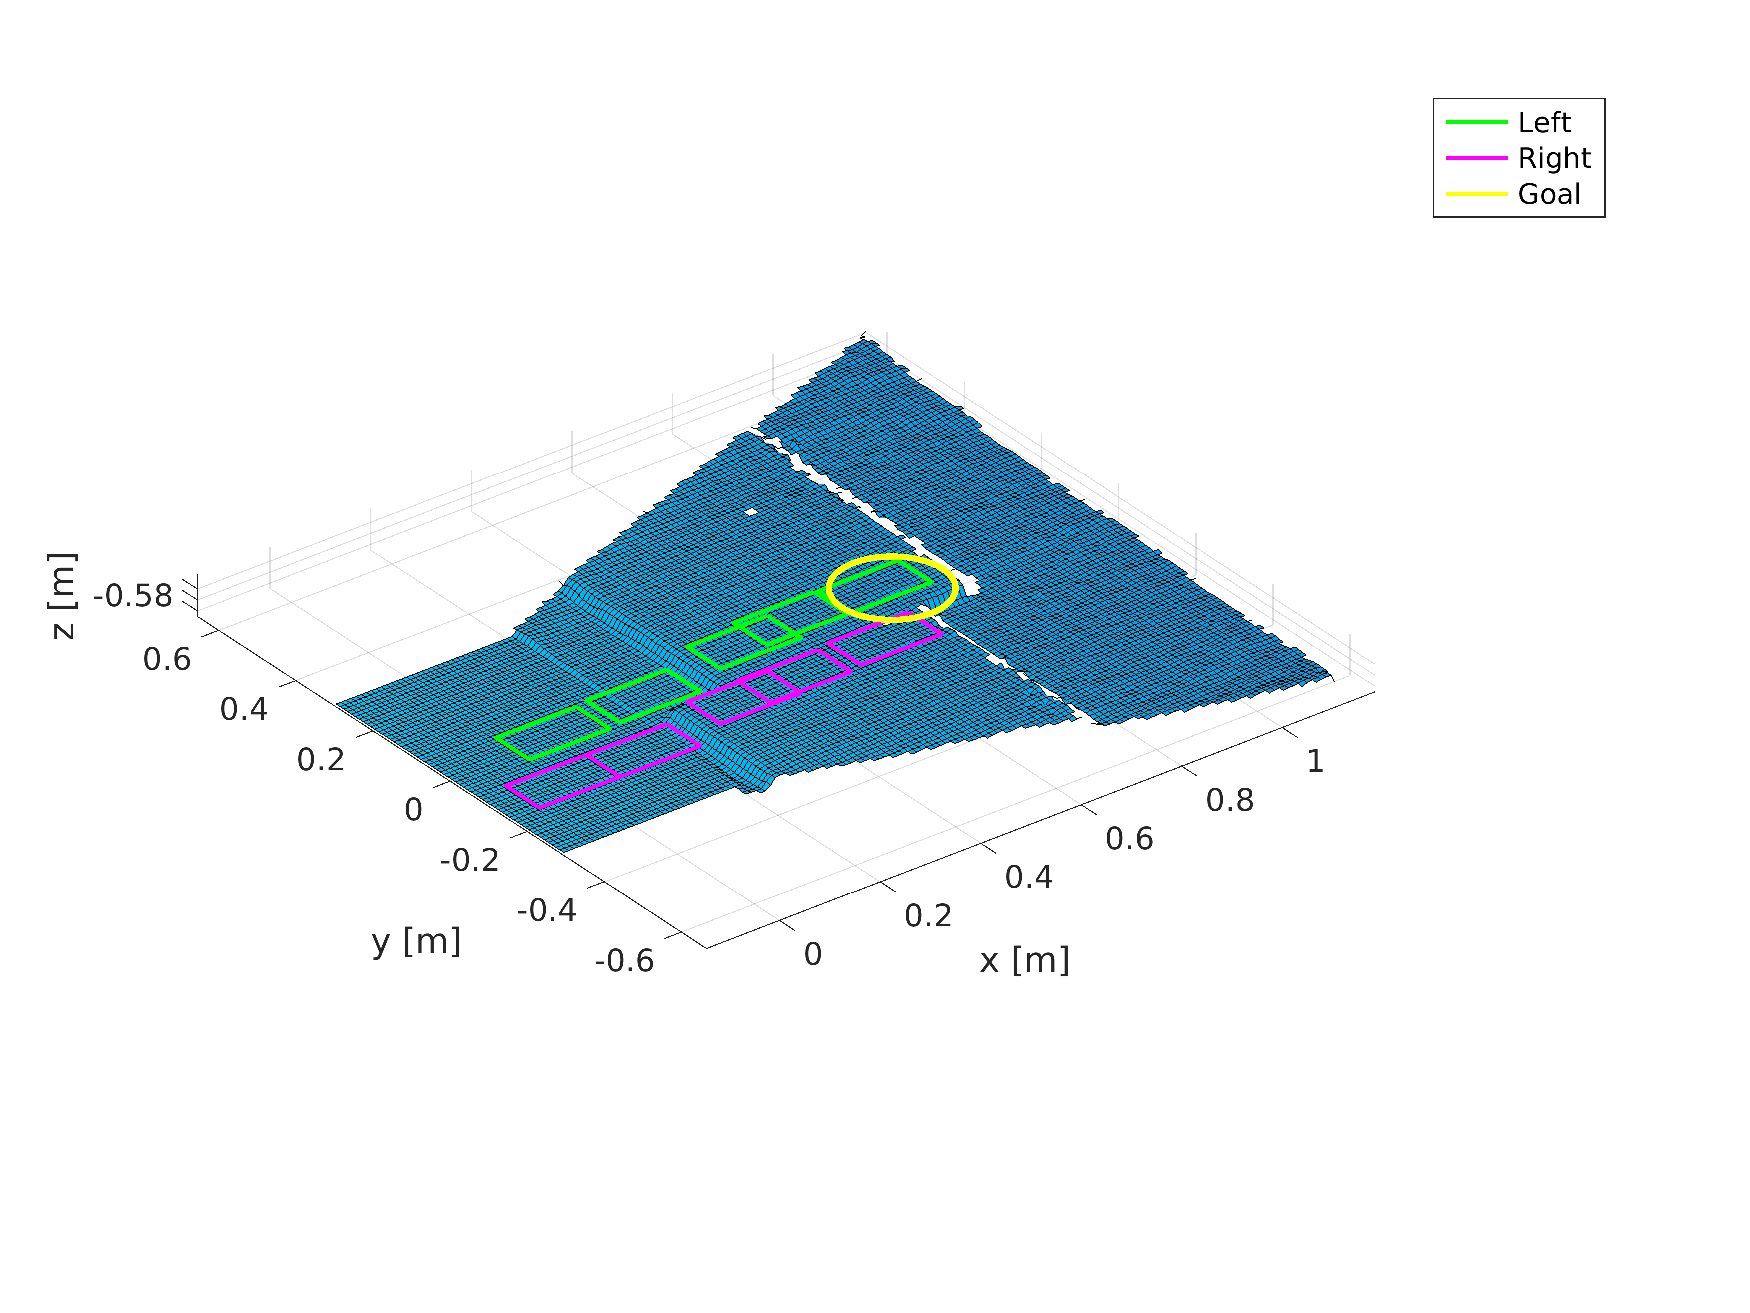
\includegraphics[width=0.95\textwidth]
        {figures/experiments/unknown-env/footstep-plan.pdf}
    \caption{Footstep plan generated for the scenario ``Stair Climbing in 
        Unknown Environments''.}
    \label{fig:experiments:unknown-env:footstep-plan}
\end{figure}
\begin{figure}
    \centering
    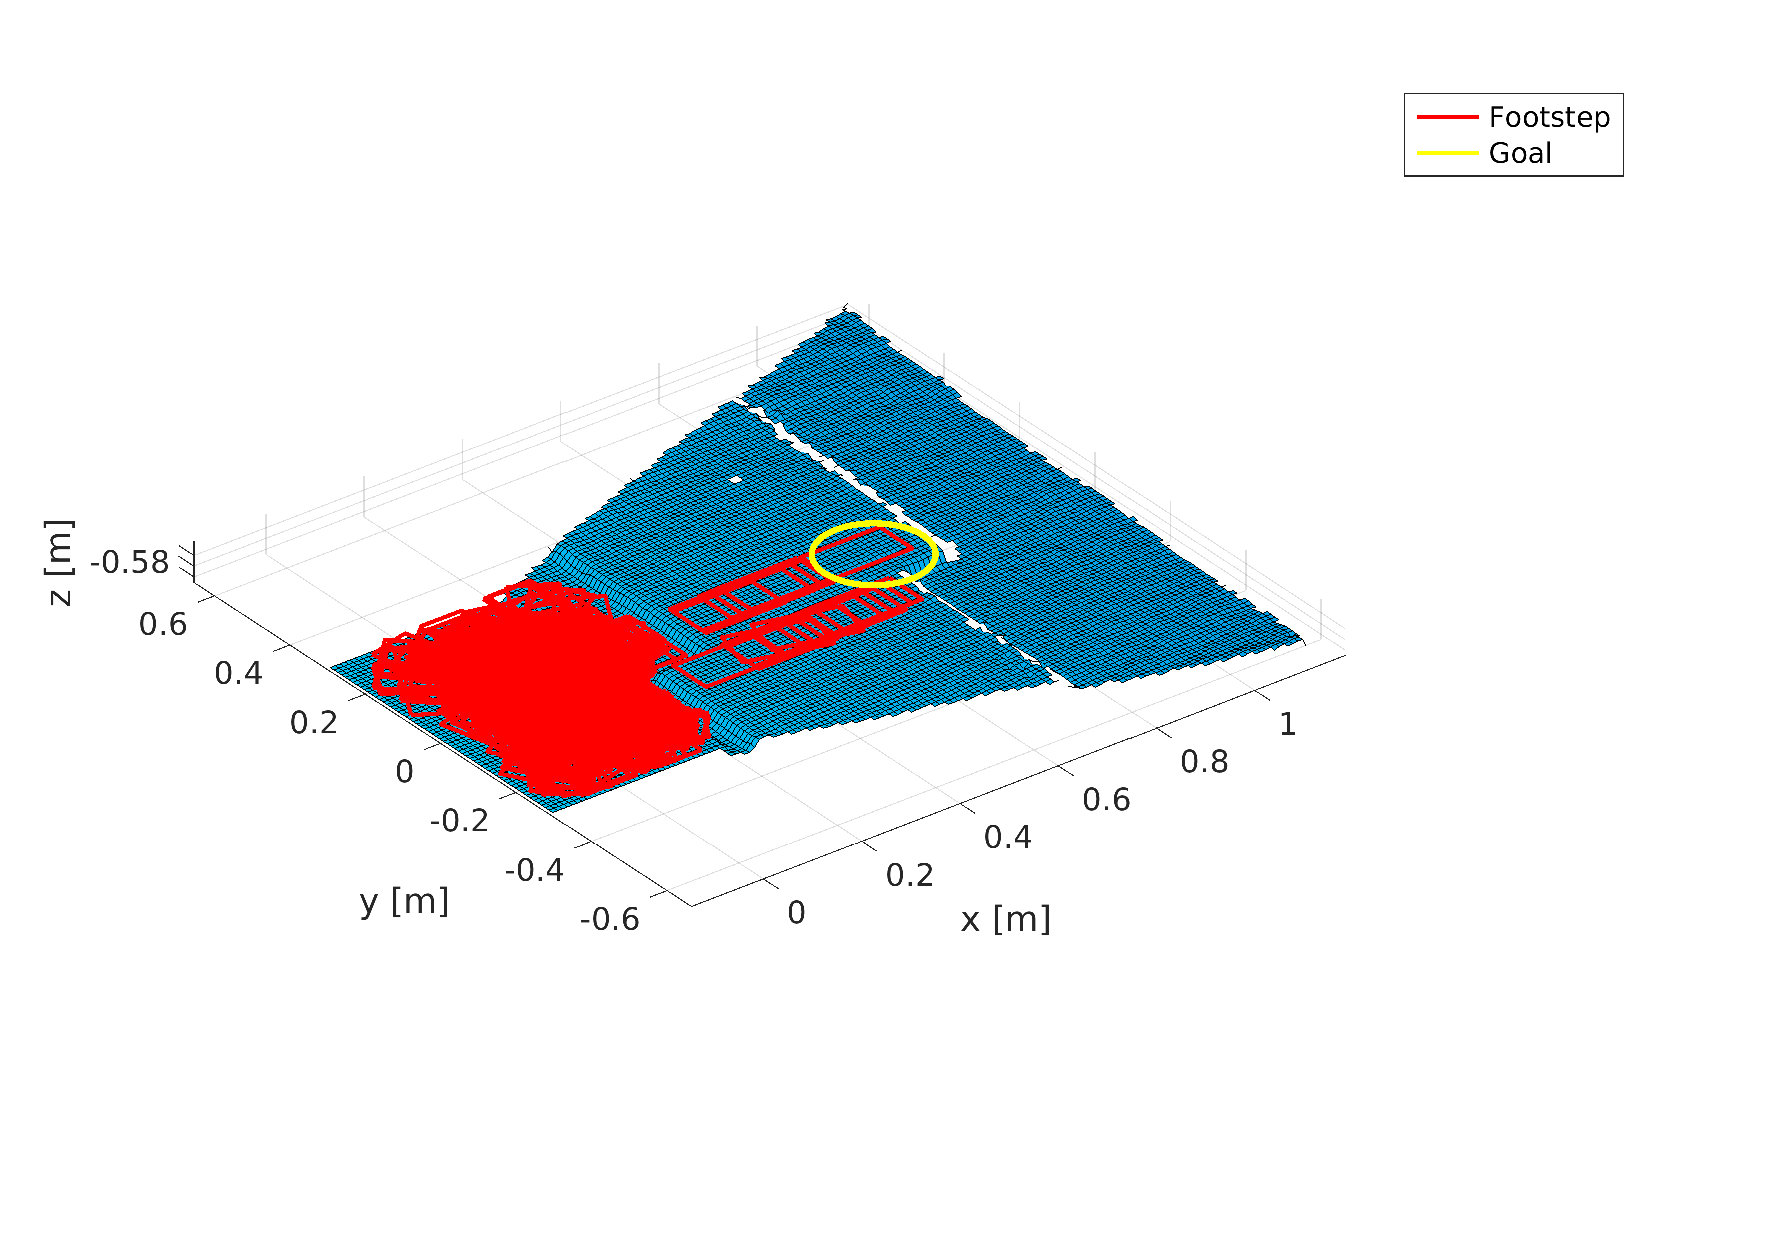
\includegraphics[width=0.95\textwidth]
        {figures/experiments/unknown-env/rrt-tree.pdf}
    \caption{Tree generated for the scenario ``Stair Climbing in 
        Unknown Environments''.}
    \label{fig:experiments:unknown-env:rrt-tree}
\end{figure}

